\chapter{Projekt rozwiązania}
\label{chap:hl-arch}

    Niniejszy rozdział przedstawia projekt systemu. Definiuje użytkowników oraz wymagania funkcjonalne i pozafunkcjonalne. Przedstawia budowę systemu, opisuje kolejno tworzące go komponenty sprzętowe oraz podsystemy, a także relacje, które między nimi zachodzą. Ponadto prezentuje zakładany sposób działania systemu w kilku najbardziej prawdopodobnych sytuacjach.

    \section{Idea}
        Idea systemu opiera się na współpracy układu zamka z serwerem w celu zapewnienia poprawnej autoryzacji identyfikatorów RFID w zamkach. Funkcjonalność autoryzacji realizowana jest wyłącznie po stronie serwera. Układ zamka, będący urządzeniem klienckim, jest jedynie pośrednikiem przekazującym dane od użytkownika do serwera. Proces ten odbywa się bezprzewodowo. Dodatkowym usprawnieniem jest zastosowanie w układzie zamka czujnika ruchu, którego zadaniem jest odpowiednio wczesne wykrycie zbliżającej się osoby i pobudzenie układu do działania. Umożliwia to przeprowadzenie czasochłonnej operacji nawiązania połączenia z serwerem autoryzacji w czasie, gdy użytkownik podchodzi do fizycznego zamka, a także oszczędzanie energii przez większą część czasu. Istotnym założeniem jest fakt, że układ operuje na zasilaniu bateryjnym. Opisywaną ideę przedstawiono na rysunku \ref{fig:door}.

        \begin{figure}[h!]
            \begin{center}
                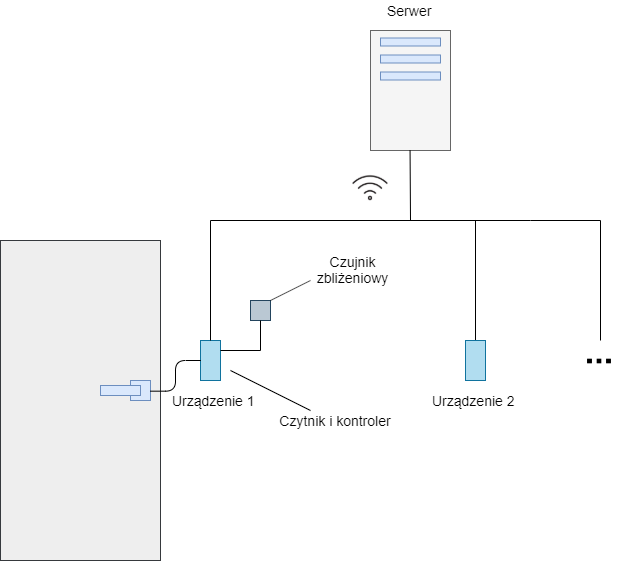
\includegraphics[width=.8\linewidth]{chapters/images/door2.png}
                \caption{Idea systemu}
                \label{fig:door}
            \end{center}
        \end{figure}

    \section{Użytkownicy}
        Na potrzeby projektu rozwiązania zidentyfikowano dwóch uniwersalnych użytkowników systemu. Ich specyfikację przedstawiono w tabeli \ref{tbl:users}.

        \begin{table}[h!]
            \caption{Użytkownicy systemu}
            \centering
            \begin{subtable}[c]{\textwidth}
                \centering
                \begin{tabular}{p{2cm}|p{12cm}}
                    USER\_1      & \textbf{Użytkownik} \\
                    \hline Opis         & Osoba posiadająca identyfikator RFID, której celem jest uzyskanie dostępu do chronionego zamkiem pomieszczenia.  \\
                \end{tabular}
                \label{tbl:usr1}
                \vspace{10mm}           
            \end{subtable}
        \quad%
            \begin{subtable}[c]{\textwidth}
                \centering
                \begin{tabular}{p{2cm}|p{12cm}}
                    USER\_2      & \textbf{Administrator} \\
                    \hline Opis         & Osoba posiadająca uprawnienia administracyjne w systemie, mająca dostęp do oprogramowania zarządzającego systemem. \\
                \end{tabular}
                \label{tbl:usr2}       
            \end{subtable}                
            \label{tbl:users}
        \end{table}

    \newpage

    \section{Wymagania}

        Wymagania funkcjonalne oraz pozafunkcjonalne systemu zostały przedstawione odpowiednio w tabeli \ref{tbl:fnrq} i \ref{tbl:xxrq}.

        \begin{table}[h!]
            \caption{Wymagania funkcjonalne}
            \centering
            \begin{subtable}[c]{\textwidth}
                \centering
                \begin{tabular}{p{2cm}|p{12cm}}
                    FNRQ\_1      & \textbf{Kontrola dostępu do pomieszczeń}  \\
                    \hline Opis         & Dopuszczanie do pomieszczeń użytkowników posiadających odpowiedni identyfikator i niedopuszczanie użytkowników nieposiadających odpowiedniego identyfikatora.  \\
                \end{tabular}
                \label{tbl:fnrq1}
                \vspace{10mm}           
            \end{subtable}
        \quad%  
            \begin{subtable}[c]{\textwidth}
                \centering
                 \begin{tabular}{p{2cm}|p{12cm}}
                    FNRQ\_2      & \textbf{Przeglądanie historii prób dostępu do pomieszczeń}  \\
                    \hline Opis         & Dostęp do listy dokonanych w przeszłości prób dostępu zakończonych zarówno sukcesem, jak i porażką. \\
                \end{tabular}
                \label{tbl:fnrq2}
                \vspace{10mm}           
            \end{subtable}
            \begin{subtable}[c]{\textwidth}
                \centering
                 \begin{tabular}{p{2cm}|p{12cm}}
                    FNRQ\_3      & \textbf{Dodawanie identyfikatorów}  \\
                    \hline  Opis         & Dodawanie identyfikatorów wraz z przyznaniem dostępu do wybranej grupy zamków. \\
                \end{tabular}
                \label{tbl:fnrq3}
                \vspace{10mm}           
            \end{subtable}
        \quad%
            \begin{subtable}[c]{\textwidth}
                \centering
                 \begin{tabular}{p{2cm}|p{12cm}}
                    FNRQ\_4      & \textbf{Przeglądanie identyfikatorów powiązanych z danym zamkiem} \\
                    \hline Opis         & Dostęp do listy powiązań między identyfikatorami a zamkami. \\
                \end{tabular}
                \label{tbl:fnrq4}
                \vspace{10mm}           
            \end{subtable}
        \quad%
            \begin{subtable}[c]{\textwidth}
                \centering
                 \begin{tabular}{p{2cm}|p{12cm}}
                    FNRQ\_5      & \textbf{Blokowanie dostępu do pomieszczeń dla wybranego identyfikatora}  \\
                    \hline Opis         & Usunięcie upoważnienia danego identyfikatora w danym zamku. \\
                \end{tabular}
                \label{tbl:fnrq5}
                \vspace{10mm}           
            \end{subtable}
        \quad%
            \begin{subtable}[c]{\textwidth}
                \centering
                 \begin{tabular}{p{2cm}|p{12cm}}
                    FNRQ\_6      & \textbf{Dostęp do grupy pomieszczeń za pomocą jednego identyfikatora}  \\
                    \hline Opis         & Ustawienie powiązań identyfikatorów i zamków w taki sposób, aby możliwy był dostęp do grupy zamków za pomocą jednego identyfikatora. \\
                \end{tabular}
                \label{tbl:fnrq6}
                \vspace{10mm}           
            \end{subtable}
        \quad%
            \begin{subtable}[c]{\textwidth}
                \centering
                 \begin{tabular}{p{2cm}|p{12cm}}
                     FNRQ\_7      & \textbf{Dostęp do pomieszczenia za pomocą grupy identyfikatorów}  \\
                    \hline Opis         & Ustawienie powiązań identyfikatorów i zamków w taki sposób, aby możliwy był dostęp do jednego zamka za pomocą grupy identyfikatorów. \\
                    \end{tabular}
                \label{tbl:fnrq7}
                \vspace{10mm}           
            \end{subtable}
        \quad%
            \begin{subtable}[c]{\textwidth}
                \centering
                 \begin{tabular}{p{2cm}|p{12cm}}
                    FNRQ\_8      & \textbf{Sygnalizacja przyznania lub odmowy dostępu}  \\
                    \hline Opis         & Powiadamianie użytkownika o podjętej przez system decyzji. \\
                \end{tabular}
                \label{tbl:fnrq8}
                \vspace{10mm}           
            \end{subtable}
            \label{tbl:fnrq}
        \end{table}

        \begin{table}[h!]
            \caption{Wymagania pozafunkcjonalne}
            \centering
            \begin{subtable}[c]{\textwidth}
                \centering
                \begin{tabular}{p{2cm}|p{12cm}}
                     XXRQ\_1      & \textbf{Długość czasu pracy układu zamka na baterii równa minimum 1 rok}  \\
                    \hline Opis         & Długość czasu pracy układu zamka na baterii powinna wynosić minimum 1 rok. \\
                \end{tabular}
                \label{tbl:xxrq1}
                \vspace{10mm}       
            \end{subtable}
        \quad%
            \begin{subtable}[c]{\textwidth}
                \centering
                \begin{tabular}{p{2cm}|p{12cm}}
                    XXRQ\_2      & \textbf{Czas odpowiedzi układu zamka nie dłuższy niż 3 sekundy}  \\
                    \hline Opis         & Czas odpowiedzi układu zamka od momentu przyłożenia identyfikatora do momentu wysłania sygnału otwierającego zamek przez układ sterowania zamkiem powinien być nie dłuższy niż 3 sekundy. \\
                \end{tabular}
                \label{tbl:xxrq2}    
            \end{subtable}
            \label{tbl:xxrq}
        \end{table}

    \vspace{10mm}

        \section{Projekt architektury}

            Na architekturę systemu składają się komponenty sprzętowe oraz podsystemy (rysunek \ref{fig:hl-arch}). Podsystemy (tabela \ref{tbl:subsystems}) realizują określone funkcjonalności za pomocą komponentów programowych (tabela \ref{tbl:sw_comp}) i istnieją w ramach komponentów sprzętowych (tabela \ref{tbl:hw_comp}). Rysunek \ref{fig:lock-arch} przedstawia szczegółową budowę układu zamka. Rysunek \ref{fig:db} przedstawia schemat bazy danych.

            \vspace{10mm}
            \begin{figure}[]
                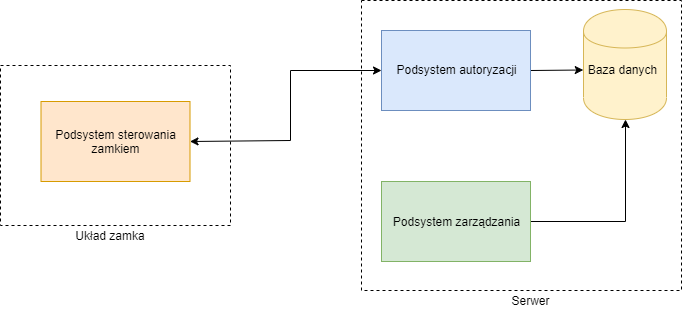
\includegraphics[width=\linewidth]{chapters/images/hl-arch3.png}
                \caption{Architektura systemu}
                \label{fig:hl-arch}
            \end{figure}

            \begin{figure}[]
                \centering
                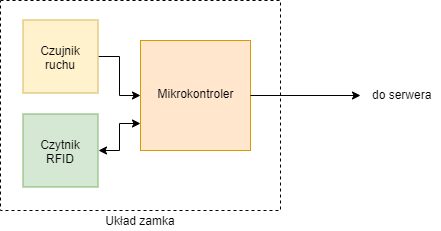
\includegraphics[width=0.5\textwidth]{chapters/images/lock.png}
                \caption{Budowa układu zamka}
                \label{fig:lock-arch}
            \end{figure}
            \vspace{10mm}
            \begin{figure}[]
                \centering
                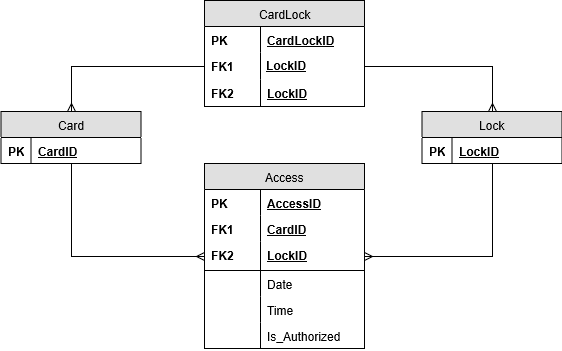
\includegraphics[width=0.8\textwidth]{chapters/images/schema.png}
                \caption{Schemat bazy danych}
                \label{fig:db}
            \end{figure}

                \begin{table}
                    \caption{Podsystemy}
                    \centering
                    \begin{subtable}[c]{\textwidth}
                        \centering
                        \begin{tabular}{p{2cm}|p{12cm}}
                            SSYS\_1      & \textbf{Podsystem sterowania zamkiem} \\
                            \hline Opis         & Odpowiedzialny za odczyt danych identyfikatora użytkownika oraz przekazanie ich do podsystemu autoryzacji, zarządzanie zasilaniem elementów układu zamka oraz zarządzanie samym zamkiem.  \\
                            \hline Lokalizacja  & HCMP\_1 Układ zamka    \\
                            \hline Komponenty   & SCMP\_1 Oprogramowanie mikrokontrolera w układzie zamka    \\
                            \end{tabular}
                        \label{tbl:scmp1}
                        \vspace{10mm}           
                    \end{subtable}
                \quad%
                    \begin{subtable}[c]{\textwidth}
                        \centering
                        \begin{tabular}{p{2cm}|p{12cm}}
                            SSYS\_2      & \textbf{Podsystem autoryzacji} \\
                            \hline  Opis         & Odpowiedzialny za podjęcie decyzji o przyznaniu bądź odmowie dostępu na podstawie otrzymanych od podsystemu sterowania zamkiem danych. Komunikuje się z podsystemem sterowania zamkiem oraz bazą danych. \\
                            \hline Lokalizacja  & HCMP\_2 Serwer    \\
                            \hline Komponenty   & SCMP\_2 Oprogramowanie autoryzujące \\
                        \end{tabular}
                        \label{tbl:ssys2}
                        \vspace{10mm}           
                    \end{subtable}
                \quad%
                    \begin{subtable}[c]{\textwidth}
                        \centering
                        \begin{tabular}{p{2cm}|p{12cm}}
                            SSYS\_3      & \textbf{Podsystem zarządzania} \\
                            \hline Opis         & Odpowiedzialny za umożliwienie administratorowi systemu wglądu do danych takich jak historia prób dostępu, zbiór identyfikatorów, zamków, oraz powiązań między nimi, a także stan poszczególnych zamków. Dzięki niemu możliwa jest konfiguracja rozpoznawanych przez system identyfikatorów i zamków oraz manualne przyznawanie dostępu poszczególnym identyfikatorom. Nazywany też podsystemem zarządzania. \\
                            \hline Lokalizacja  & HCMP\_2 Serwer    \\
                            \hline Komponenty   & SCMP\_3 Oprogramowanie zarządzające, SCMP\_4 Baza danych \\
                        \end{tabular}
                        \label{tbl:ssys3}      
                    \end{subtable}                 
                    \label{tbl:subsystems}
                \end{table}

                \begin{table}
                    \caption{Komponenty sprzętowe}
                    \centering
                    \begin{subtable}[c]{\textwidth}
                        \centering
                        \begin{tabular}{p{2cm}|p{12cm}}
                            HCMP\_1      & \textbf{Układ zamka} \\
                            \hline Opis         & Złożony z następujących subkomponentów:
                                                    \begin{itemize}
                                                        \item Mikrokontroler

                                                            Odpowiada za sterowanie peryferiami, zarządzaniem ich zasilaniem, inicjację i przeprowadzenie bezprzewodowej komunikacji z serwerem i sterowanie samym zamkiem.

                                                        \item Czujnik ruchu

                                                            Jego jedynym zadaniem jest wykrycie zbliżającego się do zamka użytkownika.

                                                        \item Czytnik RFID

                                                            Stanowi interfejs pomiędzy użytkownikiem a systemem.
                                                    \end{itemize}  \\
                            \hline Powiązania   & SCMP\_1 Oprogramowanie mikrokontrolera w układzie zamka    \\
                        \end{tabular}
                        \label{tbl:hcmp1}
                        \vspace{10mm}           
                    \end{subtable}
                \quad%
                    \begin{subtable}[c]{\textwidth}
                        \centering
                        \begin{tabular}{p{2cm}|p{12cm}}
                            HCMP\_2      & \textbf{Serwer} \\
                            \hline Opis         & Komponent na którym zlokalizowane są podsystemy autoryzacji, zarządzania oraz baza danych.  \\
                            \hline Powiązania   & SCMP\_2 Oprogramowanie autoryzujące, SCMP\_3 Oprogramowanie zarządzające, SCMP\_4 Baza danych   \\
                        \end{tabular}
                        \label{tbl:hcmp2}     
                    \end{subtable}                
                    \label{tbl:hw_comp}
                \end{table}

                \begin{table}
                    \caption{Komponenty programowe}
                    \centering
                    \begin{subtable}[c]{\textwidth}
                        \centering
                        \begin{tabular}{p{2cm}|p{12cm}}
                            SCMP\_1      & \textbf{Oprogramowanie mikrokontrolera w układzie zamka} \\
                            \hline Opis         & Odpowiedzialne za zarządzanie peryferiami układu, komunikację z serwerem oraz kontrolę zamka.  \\
                            \hline Powiązania   & HCMP\_1 Układ zamka    \\
                        \end{tabular}
                        \label{tbl:scmp1}
                        \vspace{10mm}           
                    \end{subtable}
                \quad%
                    \begin{subtable}[c]{\textwidth}
                        \centering
                        \begin{tabular}{p{2cm}|p{12cm}}
                            SCMP\_2      & \textbf{Oprogramowanie autoryzujące} \\
                            \hline Opis         & Zawiera logikę autoryzacyjną. Odbiera dane od układu zamka, komunikuje się z bazą danych w celu podjęcia decyzji o autoryzacji. \\
                            \hline Powiązania   & HCMP\_2 Serwer    \\
                        \end{tabular}
                        \label{tbl:scmp2}
                        \vspace{10mm}           
                    \end{subtable}
                \quad%
                    \begin{subtable}[c]{\textwidth}
                        \centering
                        \begin{tabular}{p{2cm}|p{12cm}}
                            SCMP\_3      & \textbf{Oprogramowanie zarządzające} \\
                            \hline Opis         & Umożliwia zarządzanie istniejącymi identyfikatorami i zamkami oraz dodawanie nowych, przeglądanie historii prób dostępu. \\
                            \hline Powiązania   & HCMP\_2 Serwer    \\
                        \end{tabular}
                        \label{tbl:scmp3}
                        \vspace{10mm}           
                    \end{subtable}                 
                \quad%
                    \begin{subtable}[c]{\textwidth}
                        \centering
                        \begin{tabular}{p{2cm}|p{12cm}}
                            SCMP\_4      & \textbf{Baza danych} \\
                            \hline Opis         & Przechowuje dane dotyczące poszczególnych identyfikatorów i zamków zarejestrowanych w systemie, powiązań pomiędzy nimi oraz dokonanych w przeszłości prób dostępu zakończonych zarówno sukcesem jak i porażką. \\
                            \hline Powiązania   & HCMP\_2 Serwer    \\
                            \end{tabular}
                        \label{tbl:scmp4}     
                    \end{subtable} 
                    \label{tbl:sw_comp}
                \end{table}

        \pagebreak

            % \begin{figure}[h!]
            %     \centering
            %     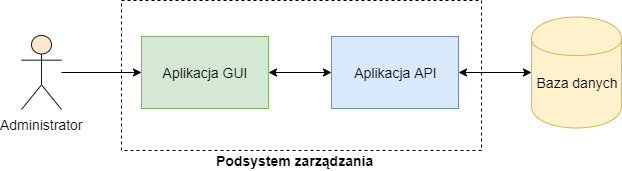
\includegraphics[width=\textwidth]{chapters/images/mngmt_subsystem.png}
            %     \caption{Budowa podsystemu zarządzania}
            %     \label{fig:mngmt_subsystem}
            % \end{figure}

        \pagebreak

        \section{Sposób działania}
            W celu osiągnięcia największej możliwej wydajności energetycznej czytnik RFID oraz mikrokontroler przez większą część czasu pozostają w stanie uśpienia. Zadaniem czujnika ruchu, zasilanego przez cały czas, jest odpowiednio wczesne wykrycie zbliżającego się użytkownika i wybudzenie mikrokontrolera, który z kolei jest odpowiedzialny za zasilenie czytnika RFID oraz nawiązanie połączenia z serwerem. Jeśli operacja nawiązania połączenia przebiegnie pomyślnie, a do czytnika przyłożony zostanie identyfikator, rozpoczyna się proces przekazywania danych odczytanych z identyfikatora do serwera w celu autoryzacji identyfikatora. Należy zwrócić uwagę na niekorzystne z punktu widzenia systemu warunki, które mogą zajść w trakcie procesu:

            \begin{enumerate}
                \item
                    Jeżeli identyfikator nie zostanie przyłożony w przeciągu 10~sek. od momentu wybudzenia czytnika, mikrokontroler ponownie wprowadza czytnik oraz samego siebie w stan uśpienia.
                \item
                    Jeżeli połączenie z serwerem nie może zostać nawiązane w czasie t + 3~sek., gdzie t jest zmiennym czasem upływającym od momentu podjęcia próby nawiązania połączenia z serwerem do momentu zakończenia odczytu danych z identyfikatora, mikrokontroler sygnalizuje użytkownikowi błąd połączenia, po czym wprowadza się w stan uśpienia.
            \end{enumerate}

            Jeżeli żadna z wymienionych wyżej niekorzystnych sytuacji nie wystąpi i dane zostaną pomyślnie przesłane do serwera, serwer podejmuje decyzję o przyznaniu bądź odmowie dostępu. Dokonuje tego po wystosowaniu zapytania do bazy danych, a następnie wysyła potwierdzenie lub odmowę do mikrokontrolera. Mikrokontroler w sposób wizualny sygnalizuje decyzję użytkownikowi, a jeżeli była ona pomyślna, dodatkowo wysyła sygnał otwierający zamek. Niezależnie od decyzji serwera, wpis o próbie dostępu zostaje zapisany w bazie danych, skąd może być pobrany przez podsystem zarządzania w celu prezentacji danych administratorowi systemu.

            Opisane wyżej mechanizmy zostały szerzej ukazane na diagramach sekwencji. Diagramy \ref{fig:sequence1}-\ref{fig:sequence3} dotyczą podsystemu sterowania zamkiem oraz podsystemu autoryzacji, natomiast diagramy \ref{fig:sequence4}-\ref{fig:sequence5} dotyczą podsystemu zarządzania.

            Przedstawione sytuacje to kolejno: proces autoryzacji identyfikatora użytkownika w przypadku najbardziej pomyślnego scenariusza (\ref{fig:sequence1}), przepływ sterowania pomiędzy elementami systemu w sytuacji, gdy użytkownik zostanie wykryty, ale identyfikator nie zostanie przyłożony do czytnika w zadanym przedziale czasu (\ref{fig:sequence2}), przepływ sterowania pomiędzy elementami systemu w sytuacji, gdy niemożliwe jest nawiązanie połączenia z serwerem (\ref{fig:sequence3}), przepływ sterowania pomiędzy warstwami podsystemu zarządzania w sytuacji żądania dostępu do historii prób dostępu przez administratora systemu (\ref{fig:sequence4}) oraz przepływ sterowania pomiędzy warstwami podsystemu zarządzajacego w sytuacji dodania nowego identyfikatora przez administratora systemu (\ref{fig:sequence5}).

            Należy zwrócić uwagę na możliwość wystąpienia również innych sytuacji niekorzystnych, takich jak błąd połączenia z bazą danych. Ich obsługa jest mało istotna z punktu widzenia współpracy komponentów systemu, dlatego nie została uwzględniona na diagramach.

            \begin{figure}[]
                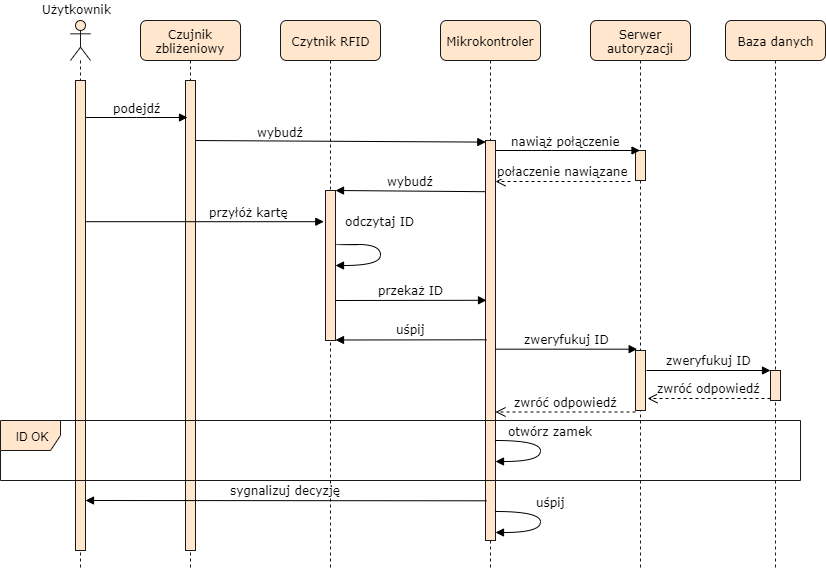
\includegraphics[width=\linewidth]{chapters/images/sequence1.png}
                \caption{Przepływ sterowania w procesie autoryzacji identyfikatora}
                \label{fig:sequence1}
            \end{figure}

            \begin{figure}[]
                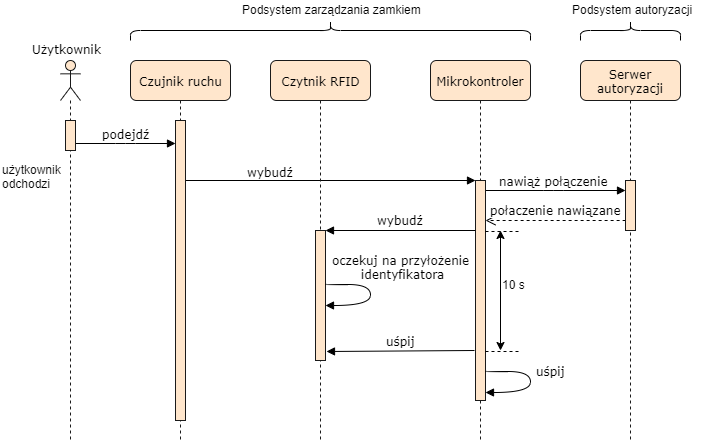
\includegraphics[width=\linewidth]{chapters/images/sequence2.png}
                \caption{Przepływ sterowania w sytuacji wykrycia użytkownika nie prezentującego identyfikatora}
                \label{fig:sequence2}
            \end{figure}

            \begin{figure}[]
                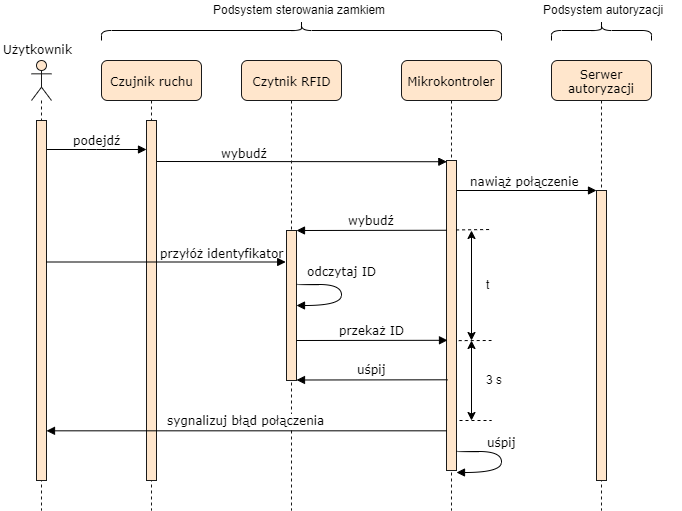
\includegraphics[width=\linewidth]{chapters/images/sequence3.png}
                \caption{Przepływ sterowania w sytuacji braku możliwości nawiązania połączenia z serwerem}
                \label{fig:sequence3}
            \end{figure}

            \begin{figure}[]
                \centering
                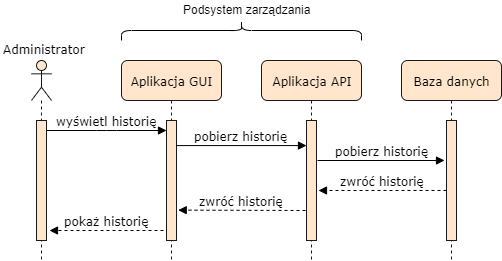
\includegraphics[width=.7\linewidth]{chapters/images/sequence4.png}
                \caption{Przepływ sterowania w procesie żądania dostępu do historii prób dostępu}
                \label{fig:sequence4}
            \end{figure}

            \begin{figure}[]
                \centering
                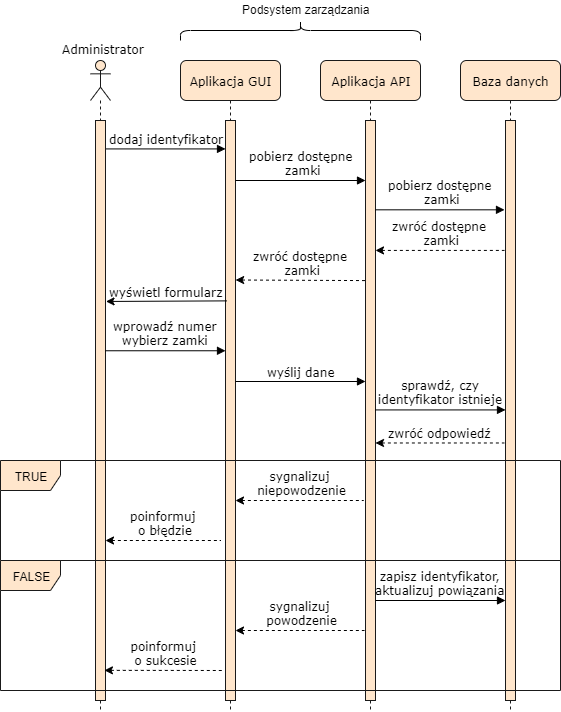
\includegraphics[width=.7\linewidth]{chapters/images/sequence5.png}
                \caption{Przepływ sterowania w procesie dodawania do systemu nowego identyfikatora}
                \label{fig:sequence5}
            \end{figure}


                    

